\subsection{ECFP feature selection}

The number of atomic environments remaining after each stage of the feature selection process is reported in Table \ref{tab:ecfp-fs}. Notably, the ratio of the number of features to the size of the training dataset is similar at
approximately \SI{74}{\%}, and so is the ratio of the initial number of features to the number of selected features, \SIrange{31}{33}{\%}. The number of features is large compared to many of the empirical models described above but not the number of graph network parameters. Furthermore, this model also aims to cover a large part of chemical space, so a large number of parameters is to be expected.

\begin{table}
    \centering
    \caption{The number of atomic environments at each stage of the ECFP feature selection process.}
    \label{tab:ecfp-fs}
    \begin{tabular}{@{}lccc@{}} \toprule
                      & \multicolumn{3}{c}{Number of training data atomic environments}                                                            \\\cmidrule(l){2-4}
        Dataset       & Initially                                                       & Found in multiple molecules & With non-negligible weight \\\midrule
        Qin-Nonionics & 260                                                             & 201                         & 81                         \\
        Qin-All       & 410                                                             & 302                         & 134                        \\\bottomrule
    \end{tabular}
\end{table}

\subsection{Hyperband tuning}

\num{725} trials were conducted for each of the Qin training datasets. The best
hyperparameters discovered on each set are described in Table \ref{tab:hb-hps}.

\begin{table}
    \centering
    \caption{The best hyperparameters discovered during searching. The $H$
        values refer to the dimensions of the corresponding layer, see Figure
        \ref{fig:model-topology}. Values for $H_{G3}$ and $H_{D2}$ have been
        omitted where the layers weren't included in the model, and the values
        of $H_P$ were only independent for the gated attention pool, so that
        they are omitted here as well.}
    \label{tab:hb-hps}
    \begin{tabular}{@{}lcc@{}} \toprule
                        & \multicolumn{2}{c}{Best value for}            \\\cmidrule(l){2-3}
        Hyperparameter  & Qin-Nonionics                      & Qin-All  \\\midrule
        \# Graph layers & 2                                  & 3        \\
        $H_{G1}$        & 320                                & 64       \\
        $H_{G2}$        & 256                                & 64       \\
        $H_{G3}$        & --                                 & 128      \\
        Pooling layer   & Mean pool                          & Sum pool \\
        $H_P$           & --                                 & --       \\
        \# Dense layers & 2                                  & 2        \\
        $H_{D1}$        & 128                                & 256      \\
        $H_{D2}$        & --                                 & --       \\\bottomrule
    \end{tabular}
\end{table}

\subsection{Model performance}

The performances of all the trained models on the test datasets are reported in Table \ref{tab:evaluation}. All of the models outperformed those of the previous work. For every task, the most accurate model was either the GNN or the combined GNN with the GP (GNN/GP). However, the linear model's performance is surprisingly good, considering its relative simplicity, faster optimisation and the far smaller number of parameters it constitutes.

\begin{table}
    \centering
    \caption{Test dataset evaluation results for the models trained in this work versus those of the previous work. The best RMSE for each task is emboldened.}
    \label{tab:evaluation}
    \begin{tabular}{@{}lccc@{}} \toprule
                                                              & \multicolumn{3}{c}{Test RMSE (\si{\log \micro M})}                                 \\\cmidrule(l){2-4}
        Model                                                 & Qin-Nonionics                                      & Qin-All       & NIST          \\\midrule
        Previous work \cite{qinPredictingCriticalMicelle2021} & 0.23                                               & 0.30          & --            \\
        ECFP                                                  & 0.19                                               & 0.26          & 1.57          \\
        GNN                                                   & \textbf{0.15}                                      & 0.29          & 1.35          \\
        GNN/GP                                                & 1.38                                               & \textbf{0.21} & \textbf{1.32} \\\bottomrule
    \end{tabular}
\end{table}

As expected, the performance of all models on the NIST data is significantly
worse than on the test data. This supports the hypothesis that the NIST data
molecules are outside of the applicability domain of the models, but it does not
exclude the possibility that the models are instead overfitted. Therefore, a more
detailed analysis of the applicability domain will be provided below.

Finally, the GNN/GP model's predictive performance on the Qin-Nonionics task was very poor. This indicates that the spacing between the molecules' latent representation vectors, determined from the corresponding GNN, was not a good
indicator of similarity with respect to CMC prediction.

\subsubsection{Uncertainty quantification}

However, the RMSE does not capture the quality of the predicted standard deviations. One metric that captures these is the negative log-likelihood (NLL) of observing the true CMCs, given the model's predicted normal distributions:
\begin{equation}
    \text{NLL} = -\sum_n \log p_n(\hat{y}_n),
\end{equation}
where subscript $n$ is the index of the data, $\hat{y}_n$ is the true CMC value and $p_n$ is the probability density function of the normal distribution $\mathcal{N}(\mu_n, \sigma_n)$, where $\mu_n$ and $\sigma_n$ are the predicted
mean and standard deviation. This metric indicates the relative performance of different models on the same data. (Note that its value scales with the size of the data.) It does not give a good indication of the quality of any individual
model in isolation, however. The NLL values are included in the supplementary information for comparison against future work.

To assess the models' quality individually, the predictions can be visualised against the true CMCs in a parity plot; see Figure \ref{fig:uq-parity}. Alternatively, a calibration plot can be used, which compares the distribution of the residuals against the expected distribution given the models' predicted normal distributions. The expected distribution simulates what would be observed if the residuals were drawn from the distributions predicted by the models.
Deviations from this distribution indicate whether the model was over- or underconfident (c.f. \citet{tranMethodsComparingUncertainty2020}). These calibration plots are shown in Figure \ref{fig:uq-calibration}.

\begin{figure}
    \centering
    \begin{subfigure}{\textwidth}
        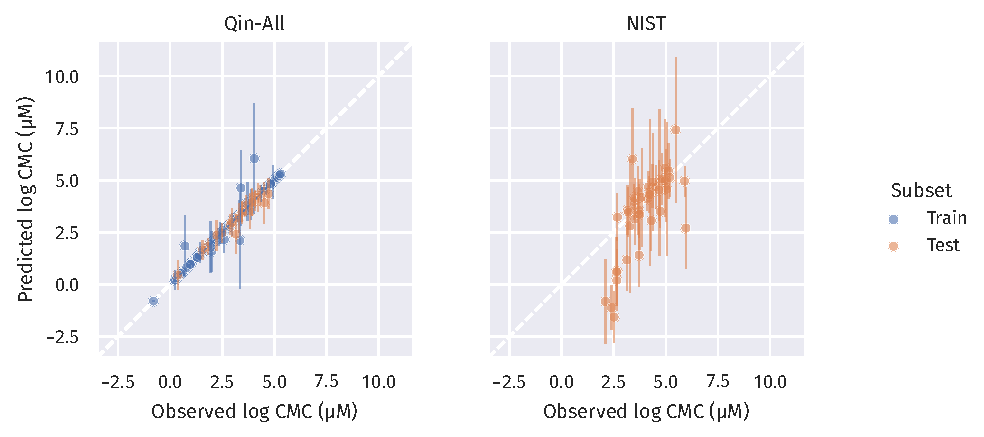
\includegraphics[width=\textwidth]{images/uq-parity.pdf}
        \caption{}
        \label{fig:uq-parity}
    \end{subfigure}
    \begin{subfigure}{\textwidth}
        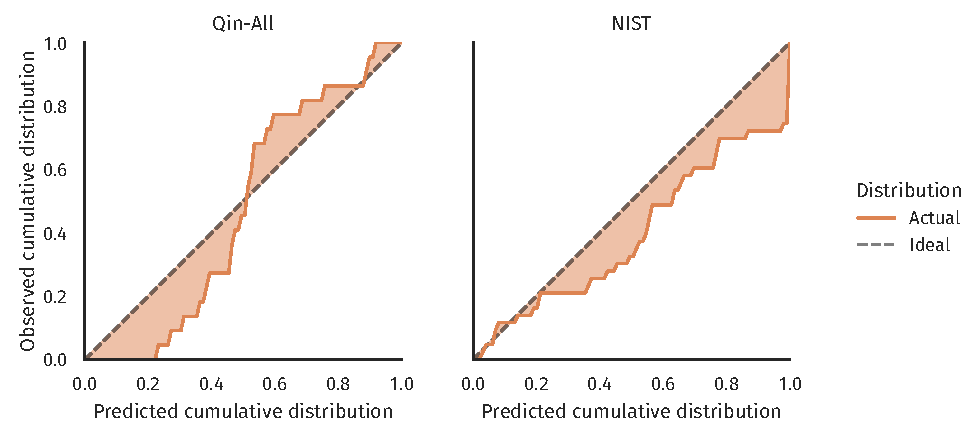
\includegraphics[width=\textwidth]{images/uq-calibration.pdf}
        \caption{}
        \label{fig:uq-calibration}
    \end{subfigure}
    \caption{(a) Parity plots of the GNN/GP model's predicted CMCs and \SI{95}{\%}
        confidence intervals for the Qin-All and NIST datasets and (b) corresponding
        calibration plots for the test data predictions.}
\end{figure}

The S-shaped calibration curve for the Qin-All test data indicates that the model was underconfident in its predictions. There is a spike in the number of observed residuals that are close to the centre of the distribution. The corresponding parity plot shows that, nevertheless, the predicted uncertainties were relatively small. The NIST data calibration curve shows remarkably good
agreement with the ideal distribution, except at the top end, which reflects the tendency of the model to underestimate the CMCs of some of the molecules. The relatively poor RMSE on the NIST data is somewhat ameliorated by the quality of
the uncertainty estimates.

Future efforts to improve this type of model may consider incorporating another term in the loss function for the GNN that explicitly biases the model towards learning a form of $\lrv{}$ that captures this similarity. Alternatively, a
variational Gaussian process could be used, which approximates the Gaussian process using a fixed-size set of `pseudo-points' \cite{hensmanGaussianProcessesBig2013a}; this would enable the entire GNN/GP model to be trained at once using backpropagation \cite{moriartyUnlockNNUncertaintyQuantification2022}.


\subsection{ECFP interpretations}

TODO: find out the hybridization states of the atoms in these fingerprints
so that we can clarify the environments more:
\begin{itemize}
    \item 4201881788
    \item 1435798937
    \item 3833245231
    \item 3204830367
\end{itemize}

The weights of the ECFP models are coefficients corresponding to the scaled counts of the selected atomic environments. Referring to Equations \ref{eq:linear-ecfp} and \ref{eq:standard-scaling}, these coefficients indicate
the change in a predicted CMC when the count of $\mathcal{E}_m$ increases by $s_m$ from its average, $u_m$. A more readily interpreted value can be achieved by rescaling the coefficient, $w_m$, for an environment:
\begin{equation}
    w_m^\prime = \frac{w_m(1 - u_m)}{s_m},
\end{equation}
which indicates the difference in predicted CMC between a molecule containing one $\mathcal{E}_m$ and a molecule without any $\mathcal{E}_m$, but which otherwise contain exactly the same number as all the other environments. This
scaled weight can be interpreted as a rough indication of the relative importance of different environments to determining CMC; `rough' because it may not be physically plausible that two molecules exist that are distinguished only
by the number of $\mathcal{E}_m$ that they contain. This is particularly true of larger environments that envelope smaller ones. The largest scaled weights for the two ECFP models are given in Table \ref{tab:env-coefs}.

\begin{table}
    \centering
    \caption{The atomic environments with the greatest importance to CMC according to the trained ECFP models.}
    \label{tab:env-coefs}
    \begin{tabular}{@{}lSlS@{}} \toprule
        \multicolumn{2}{c}{Qin-All} & \multicolumn{2}{c}{Qin-Nonionics}                                               \\\cmidrule(r){1-2}\cmidrule(l){3-4}
        Environment                 & {Scaled weight}                   & Environment               & {Scaled Weight} \\\midrule
        \ce{(CH2)5}                 & -0.64                             & \ce{(CH2)5}               & -0.76           \\
        \ce{(CH2)3}                 & -0.55                             & \ce{(CH2)3}               & -0.69           \\
        \ce{Cl-}                    & 0.31                              & \ce{(CH2)2CH}             & -0.29           \\
        \ce{Br-}                    & 0.29                              & \ce{C}                    & -0.25           \\
        \ce{(CH2)2CH}               & -0.27                             & \ce{C(CH(OH))3CH}         & -0.19           \\
        \ce{CH2}                    & -0.23                             & \ce{CH2(CH(OH))3CH}       & 0.14            \\
        \ce{O}                      & 0.18                              & \ce{CH(CH(OH))2CH2OH}     & -0.12           \\
        \ce{OH}                     & -0.17                             & \ce{CH2CH(O)(CH(OH))2CH3} & 0.09            \\
        \ce{O(CH2)2OH}              & -0.14                             & \ce{CH3}                  & -0.06           \\
        \ce{CH2O(CH2)2OH}           & -0.14                             & \ce{CH(CH(OH))3CH}        & 0.05            \\
        \bottomrule
    \end{tabular}
\end{table}

Both models agree that alkyl chain environments constitute the top two most important contributors to CMC, suggesting that tail length is the most important factor. The model trained on all surfactant classes includes two counterions in
its most important environments: \ce{Cl-} and \ce{Br-}. This is to be expected; ionic surfactants typically have much larger CMCs than nonionics, and the model appears to distinguishes these by their counterion. The Qin-Nonionics model
identifies environments from the headgroups of sugar-based surfactants as being important. These surfactant headgroups possessed relatively complex topologies and therefore several environments; it may have been necessary for the model to
use many of these environments in order to accurately distinguish between their CMCs.

TODO: Discuss NIST data and applicability domain.